% =====================================================================
%  Schematic summary of the simple-task document (proposal-simple.tex): the
%  lexical-head identification strategy. Experiments, designs tried, what works.
%  Kept up to date with each new experiment or design change.
% =====================================================================
\documentclass[10pt,a4paper]{article}

\usepackage[utf8]{inputenc}
\usepackage[T1]{fontenc}
\usepackage[margin=1.8cm]{geometry}
\usepackage{amsmath,amssymb}
\usepackage{booktabs,tabularx,array}
\usepackage{enumitem}
\usepackage{pifont}
\usepackage{xcolor}
\usepackage{xltabular}
\usepackage{tikz}
\usetikzlibrary{positioning,arrows.meta}
\usepackage[colorlinks=true,linkcolor=blue!50!black,urlcolor=blue!60!black]{hyperref}

\setlist{nosep,leftmargin=*}
\setlength{\parindent}{0pt}
\setlength{\parskip}{4pt}
\renewcommand{\arraystretch}{1.15}
\newcolumntype{L}{>{\raggedright\arraybackslash}X}

% Verdict marks
\newcommand{\yes}{\textcolor{green!45!black}{\ding{51}}}
\newcommand{\no}{\textcolor{red!70!black}{\ding{55}}}
\newcommand{\mixed}{\textcolor{orange!80!black}{$\sim$}}


\title{Lexical Task Heads on Simple Tasks\\\large Schematic project summary}
\author{Filippo Merlo}
\date{Last updated: 6 November 2026}

\begin{document}
\maketitle
\vspace{-1em}


\noindent Marks: \yes{} works / supports the hypothesis, \no{} does not, \mixed{} mixed or task-dependent. Full methods and tables: \texttt{proposal-simple.tex}. The complex tasks are summarised in \texttt{summary-complex.tex}.

% ---------------------------------------------------------------------
\section{Setup in one page}

\begin{tabularx}{\textwidth}{@{}>{\raggedright\arraybackslash\bfseries}p{2.8cm}L@{}}
\toprule
Question & Does the lexical-task-head method of Yang et al.\ (2026) reproduce on our setup, does Head-JLens (J-head) find heads the per-head logit lens (Logit-head) misses, and which heads should be kept when a task is asked for in several wordings? \\
Model & Llama-3.1-8B-Instruct (bf16; only model with released Head-JLens matrices). \\
Readouts & Logit-head: head write $c_{l,h}$ decoded by the unembedding. J-head: head output $z_{l,h}$ mapped through the fitted Jacobian $J_{l,h}$, then decoded. \\
Simple tasks & 14 Todd et al.\ tasks (antonym, capitals, translation, \dots). Rule style: the first 5 of Yang's 6 instruction templates (A--E, incl.\ the cloze form); example style: 1/5/10/20/30 shots; zero-shot prompt. Raw text, no chat template. \\
Head criterion & Head is a lexical task head on a prompt if $\geq 1$ of its top-10 tokens is in the task's term list; for the style if this holds on $\geq 10\%$ of $P^+$ (first 100 correct prompts of the most accurate wording). \\
Term lists & Yang et al.'s (2--22 token ids). Since 11-05 also lists built from the words all heads decode (J-head; E3 below). \\
Causal check 1 & Yang App.~G.1: patch the mean head output ($\times\alpha$) at the last token of prompts \emph{without} task info; control = mean of another task at the same heads. \\
Causal check 2 & Yang Sec.~2.4.1/App.~H.1.3 in their released script's setting (1-shot): patch prompts that \emph{give} the task but were answered wrongly (baseline 0). \\
Head sets patched & $H^L$, $H^J$, and J-only $H^J\setminus H^L$. \\
\bottomrule
\end{tabularx}
\medskip
\begin{center}
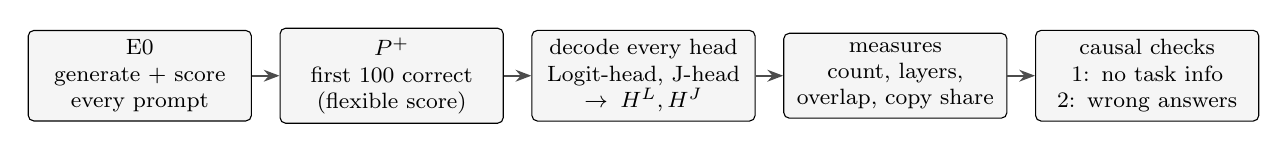
\begin{tikzpicture}[
  node distance=4mm and 3.5mm,
  box/.style={draw, rounded corners=2pt, fill=gray!8, align=center, font=\footnotesize, minimum height=9mm, text width=2.6cm},
  arr/.style={-{Stealth[length=2mm]}, thick, gray!60!black}]
\node[box] (e0) {E0\\generate + score\\every prompt};
\node[box, right=of e0] (p) {$P^{+}$\\first 100 correct\\(flexible score)};
\node[box, right=of p] (h) {decode every head\\Logit-head, J-head\\$\to H^L, H^J$};
\node[box, right=of h] (m) {measures\\count, layers,\\overlap, copy share};
\node[box, right=of m] (c) {causal checks\\1: no task info\\2: wrong answers};
\draw[arr] (e0) -- (p); \draw[arr] (p) -- (h); \draw[arr] (h) -- (m); \draw[arr] (m) -- (c);
\end{tikzpicture}
\end{center}

% ---------------------------------------------------------------------
\section{Experiments and outcomes}

\small
\begin{xltabular}{\textwidth}{@{}>{\raggedright\arraybackslash}p{2.5cm}>{\hsize=.8\hsize}L>{\hsize=1.2\hsize}Lc@{}}
\toprule
\textbf{Experiment} & \textbf{Design} & \textbf{Outcome (short)} & \\
\midrule
\endhead
\multicolumn{4}{@{}l}{\textbf{E0 --- behavioural baseline}} \\
Simple tasks & 14 tasks $\times$ 11 prompts, every item. & All tasks well above zero-shot; accuracy rises 1$\to$5 shots then flat. Template spread largest on translation, next/prev-item, park--country, synonym. & \yes \\
Scoring audit & Every reply saved; strict (first token) vs flexible vs GPT-5.5 judge; disagreement reasons. & Translation spread mostly quotes/capitals; first-token score marks any number correct. & \yes \\
\midrule
\multicolumn{4}{@{}l}{\textbf{E1 --- simple tasks} (14 tasks $\times$ rule/example $\times$ 2 readouts)} \\
Head sets & 100 prompts per style; most accurate template / 5-shot. & Logit-head finds heads on every task. J-head finds more on 23/28 pairs; its extra heads sit in layers 10--19 (Logit-head mostly $\geq$20). J-head contains all of Logit-head only on 4/28. Example heads mostly inside rule heads (70\% shared by Yang's ratio; they report 73\%). Counts within 1 head of Yang's Figs.~79/88 in their code's setting; below their Figs.~28/20. & \yes \\
Check 1 (zero-shot) & Means per wording, 15 $\alpha$ values, control mean. & Logit-head: gain $\geq$10 items on capitals, landmark, park, product (+ currency, next-item, plural with examples). Nothing on antonym, synonym, present--past, prev-item, translations. Best around $\alpha=4$. Control mostly low (not on park--country, next-item). & \mixed \\
Check 1, J-head & same & J-head $\geq$ Logit-head on most tasks; J-only heads have effects of their own. & \yes \\
Cross-style means & Rule heads $\times$ example means and vice versa. & Same tasks gain, often as much or more. & \yes \\
Check 2 (1-shot wrong) & Yang's released script, no control. & Gains on all 14 tasks; reproduces Yang's Figs.~57/62 task order. J-head far stronger on next/prev-item with examples. & \yes \\
\midrule
\multicolumn{4}{@{}l}{\textbf{E1b --- heads from several templates} (rule style, simple tasks)} \\
$k=5$ (all templates) & Heads passing under all 5 templates; both checks. & Better on fact tasks (capitals, park, product) only; worse elsewhere. Beats E1 on $\leq$5/14 tasks ($\leq$3 by $>$3 items). & \no \\
$k=1$ (union) & Exploratory. & Helps J-head on present--past (0$\to$16 items), synonym, prev-item, control flat. Hurts Logit-head on fact tasks. & \mixed \\
$k=3$ & Exploratory. & Mostly the E1 heads; behaves like E1. & -- \\
$k=1$, shared & J-head union, kept only heads in the union sets of $\geq 2$ tasks (keeps 15--62 of 19--74 heads per task); both checks. & \textbf{Not successful.} Removes most of the union's gains: present--past 16$\to$1 items (check 1), 0.64$\to$0.45 (check 2); synonym 0.21$\to$0.13. Only country--capital rises (0.60$\to$0.69). Shared heads do not carry the task better. & \no \\
$k=1$, 4 present--past heads & The 4 heads only present--past's union set contains (L19H10, L19H24, L20H28, L21H9; none in E1); both checks, present--past only. & Check 1: no effect alone (0.01); needs the other 15 heads too. Check 2: 0.63, as the whole 19-head union (0.64); rises with $\alpha$ up to 10, real past forms (60/61 distinct replies); $\alpha=0$ gives 0.02. & \mixed \\
Replies, present--past & Each patched reply sorted by kind, per head set and $\alpha$ (J-head, rule means; notebook below). & Shared heads make the model \emph{name} the task (``past tense of assess'': 65\% of replies in check 1, 73\% in check 2 at $\alpha=10$) without doing it. The 4 unshared heads make it give \emph{a form of the input}: from a bare prompt it repeats the verb (44\%), when the prompt shows the task they fix the inflection. Together (union) they give the answer. One task; heuristic reply kinds. & -- \\
Replies, all tasks & Same, every task. & Many patched replies contain the expected answer after a prefix the flexible score rejects (``Capital -- Tbilisi'', ``plural needles'', ``Country -- Russia, \dots''): 19--33\% of E1 J-head replies at $\alpha=4$ on capitals, landmark, antonym, synonym, singular--plural. Not all are answers (``opposite of solid'' for \emph{hollow}). & -- \\
Retrieval heads & Yang et al.'s retrieval heads (their code): Definition 1 with the prompt's own answer token as target, on E1's identification prompts; overlap with every lexical set, against layer-matched chance. & Mostly distinct from lexical task heads: 2--9\% of each set's heads are retrieval heads, at chance under Logit-head (0.6--1.2$\times$), slightly above under J-head (1.1--1.7$\times$, highest for $k=5$). None on the translation tasks. Of the 4 present--past unshared heads only L21H9 is one (15\% of prompts). & -- \\
4 heads split & Present--past, both checks: L21H9 (the one retrieval head of the 4) alone, and L19H10, L19H24, L20H28 alone. & L21H9 carries the effect: check 2 0.60 alone (4 heads 0.63, 3 heads 0.24); in check 1 it alone makes the model repeat the verb (44\% at $\alpha=10$), as the 4 heads do, and the 3 heads do nothing. A retrieval head that brings the input word forward; the inflection comes from the prompt's example (check 2) or the shared heads (check 1). & \mixed \\
$k=1$ without retrieval heads & $k=1$ sets (L and J) minus every retrieval head of the task (any template, either readout): 51/389 L and 84/672 J heads removed, none on translations; both checks, all tasks. & Mostly small changes, but task-dependent. Landmark--country collapses (check 1: L 0.72$\to$0.02, J 0.75$\to$0.13; J replies still name the country, not first). Present--past J loses its gains (L21H9 removed). Gains on synonym J (0.21$\to$0.32), product--company J (0.35$\to$0.48, control 0.10) and prev-item J check 2 (0.12$\to$0.45, at $\alpha$ 9--10, no constant answer). Park--country L: control now above task. Unchanged sets reproduce $k=1$ exactly. Broad removal: retrieval heads of E1's template and the same readout only would remove 12 L and 51 J heads. & \mixed \\
Equal-size sets & Top $N\in\{5,10,20\}$ heads by match rate (ties: term count) under each readout and rule (E1, $k=1/3/5$), only heads matching $\geq 1$ prompt (37/420 sets not formed); both checks, own-style means, 9 $\alpha$ ($-10,-4,2$--$6,8,10$); threshold sets compared on the same 9. & \textbf{Readouts: J-head's lead is not set size.} Of 25 threshold-set J leads $\geq 0.05$, 16 hold at every $N$, none reverse; none of Logit-head's 4 leads holds (country--capital, present--past reverse). \textbf{Rules: mostly size.} Most E1-vs-$k$ differences flip with $N$; consensus ($k=5$) below E1 in check 2 (J: antonym, singular--plural, next-item, German). No steady gain with $N$. Present--past J example: threshold (4 heads) 0.00, top 5 0.87 by adding L15H1 (rate 0.07), control 0; only sets with L15H1 move check 1. L15H1 alone (example means): 0.80 / 0.76 in checks 1 / 2 (top 5: 0.87 / 0.80; the 4 without it 0.00 / 0.57), control 0, none with rule means; J-head reads past participles from it. Control high on park--country (title starting with the country), singular--plural J ex $N=5$, next-item J ex $N=20$. & \mixed \\
Davidson FV & Davidson et al.'s (2025) instruction function vector, 4 tasks (landmark, product, English--French, present--past): heads ranked by the gain in answer probability when set to their mean on prompts whose instruction is replaced (equiprobable tokens, WikiText, other tasks' instructions), top 20 over the 4 tasks; FV = sum of their mean outputs (inst1--4, 100 prompts), added after layer 11 at the last prompt token; our check 1, 15 $\alpha$ ($\alpha=1$ is theirs), control. & Peak at $\alpha=1$ everywhere, nothing at $|\alpha|\geq 3$. Landmark 0.85, product 0.64 (controls 0.06 / 0.12; our best sets 0.79 / 0.46 at $\alpha\approx 3$--4); English--French 0.09 (control 0.03; ours $\leq$0.02); present--past 0.02 (repeats the verb, as our sets). FV heads in layers 13--17 mostly, 0--5 shared with each E1 set. English--French: 8 of the 9 hits are the English input copied where the French differs only in accents. \textbf{80 heads} (next 60 by the same score; FV 25--30\% longer, cosine 0.88--0.91 with the 20-head FV): still best at $\alpha=1$; landmark 0.96, product 0.61, English--French 0.19 (11 real translations), present--past 0.07 (real past forms); controls $\leq$0.10. \textbf{Set size} (5--1{,}024 heads, same ranking): no single best. Facts: 5--10 heads at $\alpha$ 3--4 best (landmark 0.95, product 0.87; product control 0.22), at $\alpha=1$ 40--80 heads (0.95--0.96 / 0.61). English--French: 40 heads, $\alpha=1$, 0.28 (0.20 real translations). Present--past: 320 heads, $\alpha=1$, 0.18 (real past forms). All 1{,}024 heads: facts break (0.01). Size chosen on the test items. & \mixed \\
Davidson FV, 14 tasks & As above, heads chosen over all 14 tasks (30 heads; next\_item: 12 and 28 correct prompts on two templates, so fewer for its mean); our check 1, all 14 tasks. & Best at $\alpha=1$ nearly everywhere; FV $\geq$ our best E1 set on 11/14 tasks, controls low ($\leq$0.12). Large gains where our sets do little: singular--plural 0.60 (ours $\leq$0.03), antonym 0.26 ($\leq$0.04), park--country 0.89 (0.39--0.48, our controls 0.29--0.32), English--Spanish 0.10 (real translations). Also above: capitals 0.83 (0.70), landmark 0.89, product 0.64, currency 0.13. Nothing on present--past, prev-item, synonym, English--German (0.01--0.04); English--French 0.09 = copied inputs (accents ignored). Next-item 0.10 vs J 0.17 (J control 0.35). & \mixed \\
\midrule
\multicolumn{4}{@{}p{\linewidth}@{}}{\textbf{E3 --- head sets from decoded words} (J-head only, rule style; check 1 only, rule means averaged over the 5 templates, control mean, $\alpha\in\{1,2,4,8\}$, best $\alpha$ reported. Numbers are means over the 14 tasks; E1 J-head on the same $\alpha$: 0.19.) Words: a decoded top-10 token, stripped and lowercased, kept if alphabetic, $\geq 3$ letters, not a stop word, common English (\texttt{wordfreq} Zipf $\geq 3$); \emph{share} = fraction of (prompt, head) pairs over all 1{,}024 heads whose top-10 holds it; \emph{task words} = share in the task $-$ mean share in the other 13; \emph{common words} = highest minimum share over the 14 tasks. Heads: Definition~1 with the new list ($k=10$, $\rho=0.10$) unless stated. Only $P^+$ (correct) prompts.} \\
Top decoded words & Top 40 words per task over all heads, no baseline. & Task names and answer types lead (\emph{opposite}, \emph{city}, \emph{currency}, \emph{French}); generic words on every task (\emph{what}, \emph{which}, \emph{maybe}, \emph{https}). Yang's list words only partly among them. & -- \\
Common + task, 4 tasks & 20 common and 20 task words from the best template; heads on the best template; both readouts; antonym, present--past, capitals, product. & Task list J best (capitals 0.59, antonym 0.22); common lists $\approx 0$ except product under Logit-head (0.32). & \mixed \\
All 14 tasks & Same, words counted on all 5 templates. & Task J 0.10, common J 0.07: below E1. & \no \\
List length & 5, 10, 15, 20 words. & Shorter is better: task J 0.22 (5 words) $\to$ 0.10 (20). Common $\leq 0.07$. & \mixed \\
Heads on pooled prompts & Definition~1 on the $\approx$500 prompts of the 5 templates pooled instead of the best template; also Yang's list. & Helps every list: task J 5 words 0.25; common J 0.11--0.17 (synonym 0.58 with 10 common words, control high); Yang's list pooled 0.21. & \mixed \\
Combined 5+5 ($2\times 2$) & 5 task + 5 common words; words and heads each from the best template or pooled. & \textbf{Both pooled = CC-pooled}: 0.45, 95--137 heads, above E1 on all 14 tasks; carries tasks E1 does not (antonym 0.54, singular--plural 0.64, next-item 0.43, translations 0.25--0.32). Present--past 0.03. Controls: synonym 0.26, park 0.17, singular--plural 0.12, next-item 0.12. Words pooled, heads best 0.30; words best, heads pooled 0.31; both best 0.18. & \yes \\
Random sets & Best set per task so far vs 5 layer-matched random sets of its size. & Best 0.49, random 0.03--0.07. Single draws high on antonym (0.45) and landmark (0.42); product 0.16--0.39 on all draws. & \yes \\
Strict consensus & 5+5 and 10+10 lists, head must pass on all 5 templates, top-5 tokens, $\rho=0.15$ (run at $\rho=0.05$ stopped); also its top 20 by rate. & 0.15--0.20. Best only on country--capital (0.78). & \no \\
Neutral cut (CC-pooled-clean) & J-head readings on 1{,}000 WikiText-103 passages (lengths matched); the 50 words heads read most there removed before choosing task and common words; 5+5 and 10+10, pooled. & 5+5: 0.38, 10+10: 0.33. Above CC-pooled on 8/14 (facts, translations, morphology: landmark 0.97, French 0.40, German 0.49, singular--plural 0.72, present--past 0.14). Loses antonym, synonym, next/prev-item: they need the generic words. New common words: \emph{named, therefore, question, answer, very}. & \mixed \\
Task minus WikiText & Top 10 task words after the cut; no cross-task contrast, no common words. & 0.21. Landmark 0.00 (patched replies start ``Country''), translations name the language. & \no \\
Group contrast & 5 groups (word relations, morphology, facts, sequences, translations); task words = share $-$ max share of the other tasks of its group; + 5 top WikiText words (\emph{which, mph, http, his, what}). & 0.32. Best antonym of all (0.70). Landmark and park collapse (0.01 / 0.08): \emph{country} is shared within the group and removed. & \mixed \\
Match-rate ranking & CC-pooled heads ranked by pooled match rate; top 1, 2, 5, 10, 20, 40; layer-matched random at 10, 20. & Small sets work only on capitals (L16H25 alone 0.88) and landmark (40 heads 0.93). Means: 5 heads 0.19, 20 heads 0.21, 40 heads 0.25. & \mixed \\
Relation heads & Head's top-10 holds both a term-list token and a token of the prompt's own query. & Rare: $\rho\geq 0.10$ for $\leq 7$ heads per task, none on 10 tasks. Not patched. L16H25 decodes \emph{city}, not the relation. & -- \\
Attend + decode & L16H25 pattern: at the last token it attends to \emph{capital}, \emph{country} in the instruction and decodes \emph{city}. Score = (share of last-token attention on task words in the instruction, outside the query) $\times$ (share of prompts with a task word in the J-head top 10); task words = Yang's list $\cup$ 10 top task words; eager attention, pooled prompts. Top 1, 2, 3, 5, 10, 20; layer-matched random at 5, 10. & Few heads carry fact tasks and plurals: capitals 0.88 (L16H25 alone), landmark 0.79 (5 heads), product--company 0.72 (20 heads, control 0.09; best of all), singular--plural 0.68 (20). Antonym 0.25 (5). Nothing on translations, next/prev-item, present--past. Park: control nearly as high. L16H25 ranks first on all 5 fact tasks; pattern in layers 13--17. Means: 5 heads 0.21, 20 heads 0.25 (match rate 0.19 / 0.21); random 0.04. & \mixed \\
\bottomrule
\end{xltabular}
\normalsize

% ---------------------------------------------------------------------
\section{Hypotheses}

\begin{tabularx}{\textwidth}{@{}>{\raggedright\arraybackslash}p{3.6cm}Lc@{}}
\toprule
H1 replication & Fails with the zero-shot patching of Yang App.~G.1 (check 1: no gain on 7 tasks); the G.1 figures reproduce only with check 2 (wrong prompts, Sec.~2.4.1/App.~H.1.3), which gains on all 14. & \mixed \\
H2 J-head $\supseteq$ Logit-head & Fails: J-head misses part of the Logit-head set on 24/28 pairs. J-only heads are causal in both checks. & \no \\
H3 all-template heads & Falsified: better on $\leq$5/14 tasks. & \no \\
\bottomrule
\end{tabularx}

% ---------------------------------------------------------------------
\section{Design variants tried}

\small
\begin{tabularx}{\textwidth}{@{}p{1.5cm}LLL@{}}
\toprule
\textbf{Date} & \textbf{Tried first} & \textbf{Replaced by} & \textbf{Why / effect} \\
\midrule
10-27 & Rules as main style, examples secondary & Rule and example treated alike & No main condition (user decision). \\
10-28 & Prompts and means pooled over wordings & One wording for heads, one mean per wording (Yang's code) & Matches the source exactly. \\
10-28 & Yang's batching without attention mask & Padding masked & Model attended to padding. \\
10-28 & Check 1 only (zero-shot) & Check 1 + check 2 (released script) & Only check 2 reproduces Yang's figures. \\
10-30 & First-token (simple) / strict (complex) score for heads and checks & Flexible score; E1, E2 rerun & Strict scoring created spurious wording differences. \\
11-02 & E1b with $k=5$ only & $k\in\{1,3,5\}$ & After $k=5$ failed; exploratory. \\
11-05 & Yang's hand-written term lists & Lists from decoded words (E3), J-head only & Exploratory; light check 1 ($\alpha$ 1, 2, 4, 8). \\
11-05 & Words and heads from the best template; 20-word lists & Both pooled over 5 templates; 5 + 5 words (CC-pooled) & 0.18 $\to$ 0.45; shorter lists better. \\
11-05 & Strict consensus at $\rho=0.05$ & $\rho=0.15$ & Run stopped and restarted (user decision). \\
11-05 & Common words from task prompts & Words generic text elicits removed first (WikiText) & Helps facts, translations; hurts antonym, synonym, sequences. \\
11-06 & Small sets by match rate & By attention to task words $\times$ decoding & User's L16H25 observation; larger effects at 5 and 20 heads. \\
\bottomrule
\end{tabularx}
\normalsize

\textbf{Inspecting replies:} \texttt{notebooks/patching\_outputs.py} (marimo) shows the simple-task patched replies for every manipulation: task, check, procedure (E1, $k=1/3/5$, shared/unshared), readout, head and mean style, mean source and wording, $\alpha$; accuracy, the share of the most common reply, reply kinds, and each item's replies.

% ---------------------------------------------------------------------
\section{What seems to work, what does not}

\begin{itemize}
\item \yes{} \textbf{Scoring matters first.} Flexible scoring removes most of the apparent wording sensitivity; always check it before reading wording effects.
\item \yes{} \textbf{Check 2 (wrong prompts, released-script setting)} is what reproduces Yang et al.'s figures, including those App.~G.1 attributes to zero-shot patching; the zero-shot check works only on fact-like tasks.
\item \yes{} \textbf{J-head on simple tasks:} more heads, earlier layers (10--19), and the added heads carry the task causally. It does not contain the Logit-head set.
\item \mixed{} \textbf{Which heads to keep} depends on the task type: all-template heads for fact tasks, union of templates for morphology-like tasks under J-head.
\item \mixed{} \textbf{Retrieval heads} (heads that already write the answer token) are few among lexical task heads, but some effects rest on them: landmark--country's on its 10, present--past's union gain on L21H9. Elsewhere removing them changes little or helps (synonym, product--company, prev-item under J-head). Entity-answer tasks may be carried by retrieval more than by task heads.
\item \mixed{} \textbf{Two roles on present--past} (one task): heads shared across tasks make the model \emph{name} the task; L21H9 makes it give \emph{a form of the input}. Either alone fails from a bare prompt; with an example in the prompt, L21H9 alone suffices.
\item \yes{} \textbf{J-head vs Logit-head at equal size:} J-head's larger effects mostly remain with 5, 10 or 20 heads per readout; Logit-head's few leads do not. Differences between template rules mostly come from set size.
\item \yes{} \textbf{Words the heads actually decode make better lists} (J-head, check 1): CC-pooled (5 task + 5 common words, words and heads over all 5 templates) is above E1 on all 14 tasks (mean 0.45 vs 0.19) and carries antonym, singular--plural, next-item and the translations, where E1 does nothing. Both word kinds and the pooling are needed.
\item \mixed{} \textbf{Generic words help some tasks.} Removing the words heads read on any text (WikiText) helps facts, translations and morphology but hurts antonym, synonym and sequences.
\item \mixed{} \textbf{Few heads suffice for named answer types:} heads that attend to the instruction's task words and decode the answer type carry capitals (1 head), landmark (5), product--company and singular--plural (20). Not translations, sequences, present--past.
\item \textbf{E3 caveats:} words, list sizes and designs chosen after seeing check 1 on the same items; best of 4 $\alpha$; one run; no check 2, no held-out items yet.
\item \textbf{Read the replies, not only accuracy:} 19--33\% of patched replies on several tasks contain the answer after a prefix the flexible score rejects, and part of a ``loss'' can be a format change (landmark--country under J-head). \texttt{notebooks/patching\_outputs.py} shows them.
\end{itemize}

\textbf{Not pursued:} function vectors, function-specific heads, hidden-state differences (scope, 10-27); fp32 Head-JLens fit ($\approx$136 GPU-h, declined); hand-labelled validation of the judge.

\end{document}
